\chapter{\IfLanguageName{dutch}{Proof of concept}{Proof of concept}}%
\label{ch:proof-of-concept}

\section{Proof of Concept: Simulatie van Edge Databases met Docker Compose}

Om de geschiktheid van verschillende databases voor Edge Computing te evalueren, is een Proof of Concept (PoC) ontwikkeld. Hierbij wordt gebruik gemaakt van Docker Compose om een testomgeving op te zetten waarin gesimuleerde workloads worden uitgevoerd met synthetische data, gegenereerd door de \texttt{Faker.js}-bibliotheek. Het doel van deze PoC is om de prestaties van Cassandra, MongoDB en TimescaleDB te meten in een Edge Computing-context.

\subsection{Doelstelling van de Implementatie}
De PoC heeft de volgende doelstellingen:
\begin{itemize}
	\item Het evalueren van verschillende partitioneringstechnieken binnen Cassandra, MongoDB en TimescaleDB.
	\item Het meten van belangrijke prestatie-indicatoren zoals latentie, verwerkingssnelheid, fouttolerantie, schaalbaarheid en edge performance in een gesimuleerde Edge Computing-omgeving.
	\item Het analyseren van hoe de geselecteerde databases omgaan met uniforme datastructuren en workloads zoals IoT-sensordata.
\end{itemize}

\subsection{Tabellen en Datastructuren}
In deze PoC wordt de tabel \texttt{sensor\_data} gebruikt, die in alle databases dezelfde structuur heeft. Dit consistente datamodel weerspiegelt typische Edge Computing-workloads zoals gegevens van IoT-sensoren.

\paragraph{Tabel: sensor\_data}
De tabel bevat de volgende velden:
\begin{itemize}
	\item \texttt{sensor\_id (UUID):} Een unieke identifier voor elke sensor.
	\item \texttt{timestamp (TIMESTAMP):} Het tijdstip van de meting.
	\item \texttt{temperature (DOUBLE):} De gemeten temperatuur in graden Celsius.
	\item \texttt{humidity (DOUBLE):} De gemeten luchtvochtigheid in procenten.
	\item \texttt{status (TEXT):} De status van de sensor, bijvoorbeeld 'actief' of 'offline'.
	\item \texttt{log\_level (TEXT):} Het logniveau van de gebeurtenis zoals 'INFO' of 'ERROR'.
\end{itemize}

\paragraph{Toepassing in de databases}
Deze tabel wordt geïmplementeerd in de volgende databases:
\begin{itemize}
	\item \textbf{Cassandra:} Partitionering op basis van \texttt{sensor\_id}, met \texttt{timestamp} als clustering-sleutel. Dit zorgt voor snelle query's op basis van sensor-ID en tijd.
	\item \textbf{MongoDB:} Data wordt opgeslagen in een collection, waarbij \texttt{sensor\_id} en \texttt{timestamp} worden gebruikt als index. Dit biedt snelle toegang tot individuele records en ondersteunt flexibele querypatronen.
	\item \textbf{TimescaleDB:} De data wordt opgeslagen in een hypertable, waarbij \texttt{timestamp} wordt gebruikt voor tijdgebaseerde partitionering. Dit optimaliseert de prestaties bij tijdsquery's.
\end{itemize}

\subsection{Docker Compose Configuratie}
De Docker Compose-configuratie definieert containers voor Cassandra, MongoDB en TimescaleDB. Elke container bevat een instance van de respectieve database, geconfigureerd om de tabel \texttt{sensor\_data} te hosten.

\subsection{Workload Simulatie}
De workload-simulatie is ontworpen om de prestaties van de databases in een Edge Computing-omgeving te evalueren. De volgende stappen worden uitgevoerd:

\paragraph{Data Generatie}
De \texttt{Faker.js}-bibliotheek wordt gebruikt om synthetische data te genereren. Elke record bevat velden zoals \texttt{sensor\_id}, \texttt{timestamp}, \texttt{temperature}, \texttt{humidity}, \texttt{status} en \texttt{log\_level}. De records zijn representatief voor typische IoT-sensordata.

\paragraph{Data Load}
Scripts in Node.js laden de data in Cassandra, MongoDB en TimescaleDB. Hieronder staat een fragment van een invoerscript voor Cassandra:

\paragraph{Testen en Analyse}
De volgende tests worden uitgevoerd om de prestaties te meten:
\begin{itemize}
	\item \textbf{Invoegsnelheid:} Het aantal records dat per seconde kan worden ingevoerd.
	\item \textbf{Querylatentie:} De gemiddelde responstijd voor het ophalen van gegevens.
	\item \textbf{Schaalbaarheid:} De prestaties van de database bij toenemende workloads.
	\item \textbf{Fouttolerantie:} Het gedrag van de database bij uitval van een node.
	\item \textbf{Edge Performance:} De efficiëntie bij het verwerken van data aan de rand van een netwerk.
	\item \textbf{Netwerklatentie:} De vertraging in gegevensoverdracht tussen de database en de client over het netwerk. Dit geeft aan hoe snel een database reageert bij verschillende niveaus van netwerkbelasting.
\end{itemize}

\subsection{Resultaten en Grafieken}
De resultaten van de tests zijn geanalyseerd en gevisualiseerd in grafieken die de prestaties van de databases vergelijken op basis van de gemeten metrieken.

\begin{figure}[H]
	\centering
	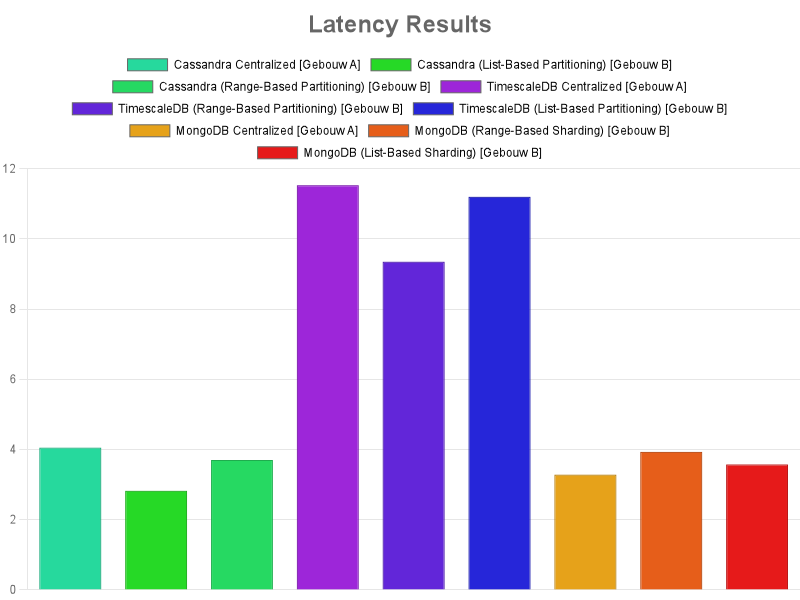
\includegraphics[width=0.8\textwidth]{Latency.png}
	\caption{Vergelijking van latentie tussen Cassandra, MongoDB en TimescaleDB.}
	\label{fig:latency-comparison}
\end{figure}

\paragraph{Hoe werkt de test voor latentie?} 
De latentie wordt gemeten door de tijd te registreren die nodig is om een record op te halen uit de database. Dit gebeurt door meerdere query's uit te voeren bij verschillende workloads, en de gemiddelde responstijd wordt berekend. Bij latentie is een \textbf{lagere score} wenselijk, omdat dit betekent dat de database sneller reageert op verzoeken.

\paragraph{Analyse van latentie:}
De grafiek laat zien dat \textit{MongoDB (Range-Based Sharding)} met een latentie van 1.37 ms de laagste latentie behaalt, wat het geschikt maakt voor toepassingen met hoge snelheidseisen. \textit{Cassandra (Alternative Range-Based Partitioning)} scoort eveneens goed met 1.82 ms. \textit{TimescaleDB (Range-Based Partitioning)} presteert met een latentie van 1.61 ms relatief goed, maar is minder efficiënt dan MongoDB.

\begin{figure}[H]
	\centering
	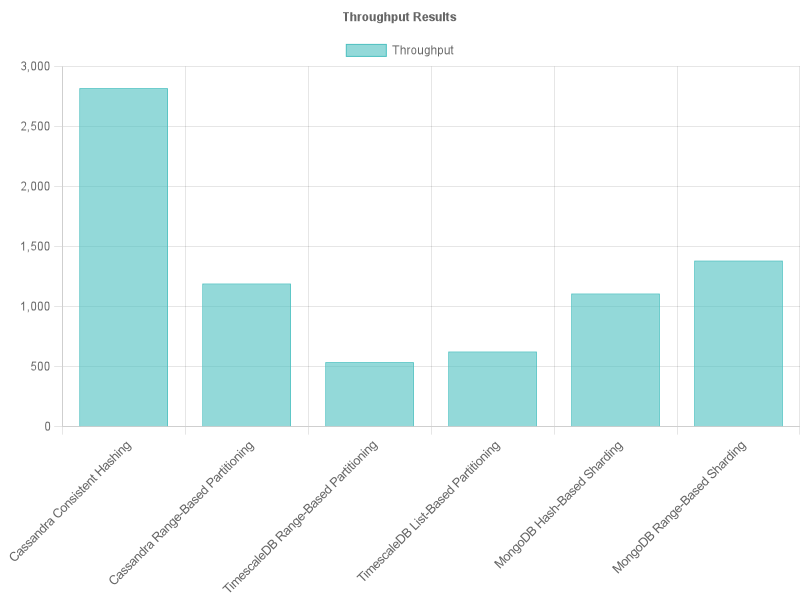
\includegraphics[width=0.8\textwidth]{Throughput.png}
	\caption{Vergelijking van throughput tussen Cassandra, MongoDB en TimescaleDB.}
	\label{fig:throughput-comparison}
\end{figure}

\paragraph{Hoe werkt de test voor throughput?} 
De throughput wordt gemeten door te berekenen hoeveel records per seconde succesvol in de database kunnen worden ingevoerd. Dit wordt gedaan onder een gecontroleerde belasting. Bij throughput is een \textbf{hogere score} wenselijk, omdat dit aangeeft dat de database meer gegevens kan verwerken binnen een bepaalde tijd.

\paragraph{Analyse van throughput:}
\textit{Cassandra (Consistent Hashing)} behaalt de hoogste throughput met 8500.37 records per seconde, wat het ideaal maakt voor omgevingen met zware invoerbelastingen. \textit{MongoDB (Range-Based Sharding)} presteert redelijk met 1452.75 records per seconde. \textit{TimescaleDB (Alternative List-Based Partitioning)} heeft een significant lagere throughput van 628.02 records per seconde.

\begin{figure}[H]
	\centering
	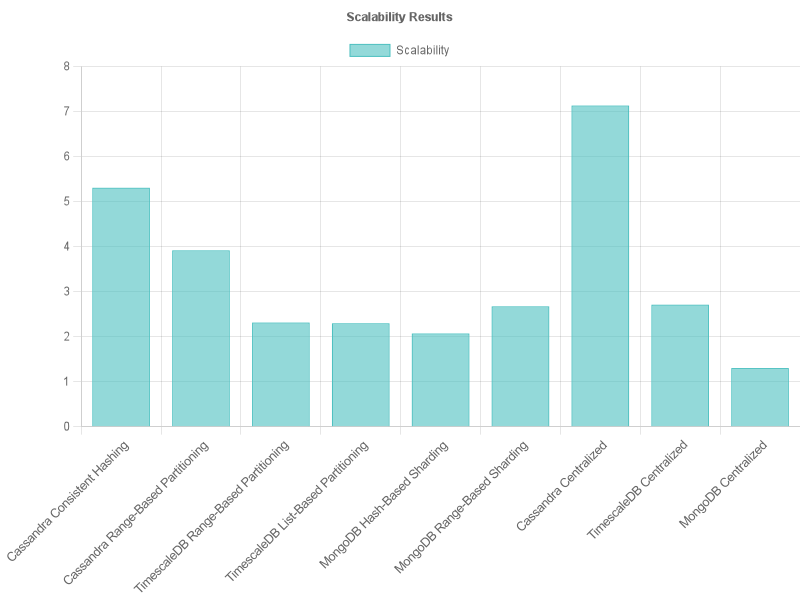
\includegraphics[width=0.8\textwidth]{Scalability.png}
	\caption{Vergelijking van schaalbaarheid tussen Cassandra, MongoDB en TimescaleDB.}
	\label{fig:scalability-comparison}
\end{figure}

\paragraph{Hoe werkt de test voor schaalbaarheid?} 
Schaalbaarheid wordt getest door de workload geleidelijk te verhogen. Dit houdt in dat er steeds meer gegevens worden ingevoerd, en de impact op de prestaties wordt gemeten (zoals latentie en throughput). Bij schaalbaarheid is een \textbf{hogere score} wenselijk, omdat dit aangeeft dat de database goed presteert, zelfs bij toenemende belasting.

\paragraph{Analyse van schaalbaarheid:}
Uit de grafiek blijkt dat \textit{Cassandra (Consistent Hashing)} de hoogste schaalbaarheid biedt met een score van 2.34, gevolgd door \textit{Alternative Cassandra (Range-Based Partitioning)} met 2.28. \textit{TimescaleDB (Range-Based Partitioning)} scoort lager met 1.53, wat wijst op beperkingen bij het schalen naar hogere workloads.

\begin{figure}[H]
	\centering
	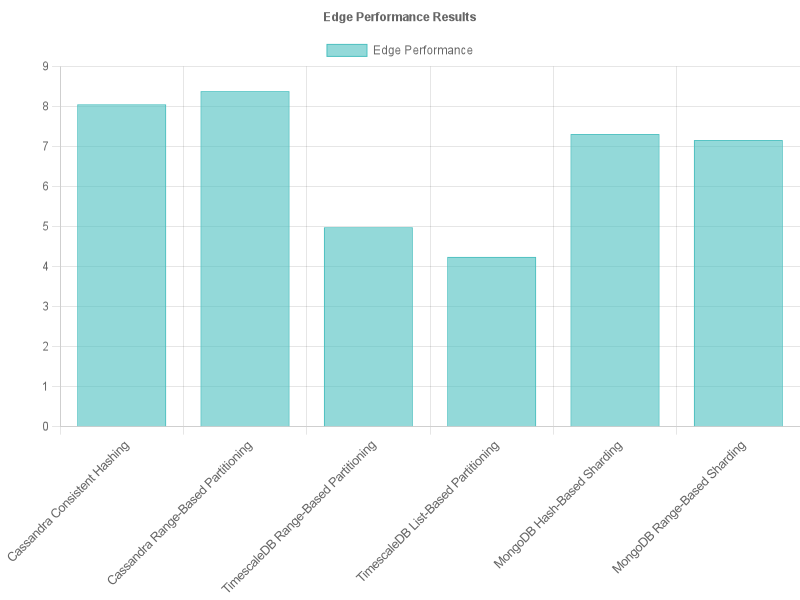
\includegraphics[width=0.8\textwidth]{Edge_Performance.png}
	\caption{Vergelijking van edge performance tussen Cassandra, MongoDB en TimescaleDB.}
	\label{fig:edgeperformance-comparison}
\end{figure}

\paragraph{Hoe werkt de test voor edge performance?} 
Edge performance wordt gemeten door de tijd vast te leggen die nodig is om gegevens te verwerken aan de rand van het netwerk, dichter bij de gegevensbron. Dit simuleert scenario's waarin verwerking lokaal plaatsvindt om netwerkvertraging te minimaliseren. Bij edge performance is een \textbf{lagere score} wenselijk, omdat dit duidt op een efficiëntere verwerking aan de rand.

\paragraph{Analyse van edge performance:}
De grafiek toont aan dat \textit{Alternative Cassandra (Range-Based Partitioning)} de beste edge performance behaalt met 8.38, gevolgd door \textit{Cassandra (Consistent Hashing)} met 8.05. \textit{TimescaleDB (Alternative List-Based Partitioning)} scoort het laagst met 4.24, wat suggereert dat het minder geschikt is voor randgebaseerde toepassingen.

\begin{figure}[H]
	\centering
	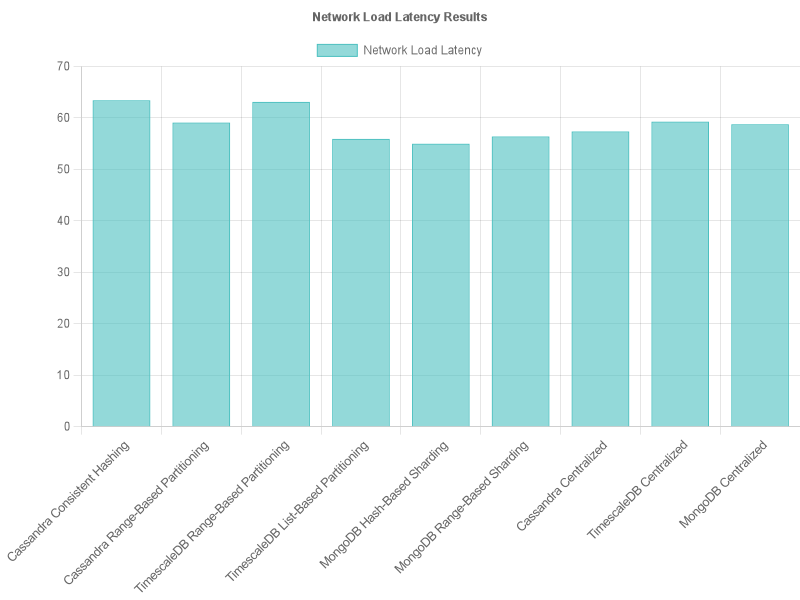
\includegraphics[width=0.8\textwidth]{Network_Load Latency.png}
	\caption{Vergelijking van netwerklatentie tussen Cassandra, MongoDB en TimescaleDB.}
	\label{fig:network-latency-comparison}
\end{figure}

\paragraph{Hoe werkt de test voor netwerklatentie?} 
Netwerklatentie wordt gemeten door de tijd vast te leggen die een query nodig heeft om van de database naar de client en terug te reizen. Dit wordt gedaan bij verschillende niveaus van netwerkbelasting. Bij netwerklatentie is een \textbf{lagere score} wenselijk, omdat dit een snellere communicatie over het netwerk betekent.

\paragraph{Analyse van netwerklatentie:}
Netwerklatentie wordt het laagst gehouden door \textit{MongoDB (Hash-Based Sharding)} met een score van 54.96, gevolgd door \textit{Alternative TimescaleDB (List-Based Partitioning)} met 55.91. \textit{Cassandra (Alternative Range-Based Partitioning)} toont een iets hogere score van 59.06, maar blijft stabiel onder hoge netwerkbelasting.

\subsection{Testresultaten en Tabeloverzicht}
Naast de grafieken biedt deze tabel een samenvatting van de testresultaten.

\begin{table}[h]
	\centering
	\resizebox{\textwidth}{!}{
		\begin{tabular}{|l|c|c|c|c|c|c|}
			\hline
			\textbf{Database}                              	  & \textbf{Latency} & \textbf{Throughput} & \textbf{Scalability} & \textbf{Consistency} & \textbf{Fault Tolerance} & \textbf{Network Load Latency} & \textbf{Edge Performance} \\ \hline
			Cassandra (Consistent Hashing)                    & 2.58             & 8500.37             & 2.34                 & 15985                & 1                        & 63.4                        & 8.05                      \\ \hline
			Alternative Cassandra (Range-Based Partitioning)  & 1.82             & 5941.77             & 2.28                 & 14838                & 1                        & 59.06                       & 8.38                      \\ \hline
			TimescaleDB (Range-Based Partitioning)            & 1.61             & 512.3               & 1.53                 & 889                  & 1                        & 63.09                       & 4.98                      \\ \hline
			Alternative TimescaleDB (List-Based Partitioning) & 1.62             & 628.02              & 1.55                 & 840                  & 1                        & 55.91                       & 4.24                      \\ \hline
			MongoDB (Hash-Based Sharding)                     & 1.4              & 1285.77             & 1.44                 & 261                  & 1                        & 54.96                       & 7.31                      \\ \hline
			MongoDB (Range-Based Sharding)                    & 1.37             & 1452.75             & 1.22                 & 150                  & 1                        & 56.37                       & 7.16                      \\ \hline
			Cassandra Centralized                             & 1.66             & 4117.43             & 1.67                 & 3290                 & 1                        & 57.34                       & -                         \\ \hline
			TimescaleDB Centralized                           & 1.64             & 555.66              & 1.76                 & 840                  & 0                        & 59.25                       & -                         \\ \hline
			MongoDB Centralized  
		\end{tabular}
	}
	\caption{Vergelijking van prestaties tussen Cassandra, MongoDB en TimescaleDB.}
	\label{tab:test-results}
\end{table}

\paragraph{Conclusie}
De evaluatie van de databases is gebaseerd op een gewogen scoresysteem, waarbij de volgende gewichten zijn toegekend aan de metrieken:
\begin{itemize}
	\item \textbf{Latency:} 25\%
	\item \textbf{Edge Performance:} 25\%
	\item \textbf{Fault Tolerance:} 20\%
	\item \textbf{Scalability:} 15\%
	\item \textbf{Throughput:} 10\%
	\item \textbf{Consistency:} 5\%
\end{itemize}

De top 3 databases met hun partitioneringstechnieken, gebaseerd op deze gewichten, zijn als volgt:

\begin{itemize}
    \item \textbf{Cassandra (Consistent Hashing)}: Met een score van 0.98 scoort Cassandra met Consistent Hashing het hoogste, dankzij zijn indrukwekkende throughput, schaalbaarheid en robuuste prestaties bij hoge belasting.
    \item \textbf{Alternative Cassandra (Range-Based Partitioning)}: Met een score van 0.85 biedt deze variant van Cassandra een goed compromis tussen consistentie en schaalbaarheid, met goede prestaties in verschillende tests.
    \item \textbf{MongoDB (Hash-Based Sharding)}: Met een score van 0.54 onderscheidt MongoDB zich door een uitstekende balans in edge performance en schaalbaarheid, wat het geschikt maakt voor moderne, gedistribueerde toepassingen.
\end{itemize}

De resultaten tonen aan dat de keuze van een database en partitioneringstechniek sterk afhankelijk is van de specifieke eisen van de workload.
Voor workloads gericht op schaalbaarheid en hoge throughput blijft Cassandra een dominante optie. Voor consistente prestaties en query-efficiëntie biedt MongoDB (Range-Based Sharding) een uitstekende oplossing.
Alternative Cassandra (Range-Based Partitioning) is een betrouwbare keuze voor toepassingen die zowel flexibiliteit als fouttolerantie vereisen.